% !TeX program = pdflatex
% !TeX encoding = UTF-8
% !TeX spellcheck = pt_BR
\documentclass[
  article,
  11pt,
  a4paper,
  english,
  brazil,
  sumario=tradicional]{abntex2}
\usepackage{lmodern}			% Usa a fonte Latin Modern
\usepackage[T1]{fontenc}		% Seleção de códigos de fonte.
\usepackage[utf8]{inputenc}		% Codificação do documento (conversão automática dos acentos)
\usepackage{indentfirst}		% Indenta o primeiro parágrafo de cada seção.
\usepackage{nomencl} 			% Lista de simbolos
\usepackage{color}				% Controle das cores
\usepackage{graphicx}			% Inclusão de gráficos
\usepackage{microtype} 			% Melhorias de justificação
\usepackage{csquotes}			% Aspas e citações mais simples
\usepackage{booktabs}			% Tabelas mais profissionais

% ---
% Pacotes de citações
% ---
\usepackage[brazilian,hyperpageref]{backref}	 % Paginas com as citações na bibliografia
\usepackage[alf]{abntex2cite}	% Citações padrão ABNT
% ---

% ---
% Configurações do pacote backref
% Usado sem a opção hyperpageref de backref
\renewcommand{\backrefpagesname}{Citado na(s) página(s):~}
% Texto padrão antes do número das páginas
\renewcommand{\backref}{}
% Define os textos da citação
\renewcommand*{\backrefalt}[4]{
  \ifcase #1 %
  Nenhuma citação no texto.%
  \or
  Citado na página #2.%
  \else
  Citado #1 vezes nas páginas #2.%
  \fi}%
% ---

% Para fórmulas matemáticas
\usepackage{amsmath}
\usepackage{amssymb}
\usepackage{mathtools}

% Para setas usadas em fórmulas dos grafos
\usepackage{MnSymbol}

% Diretório padrão para figuras
\graphicspath{ {images/} }

% Permite colocar figuras lado a lado ou
% fazer posicionamentos arbitrários
\usepackage[lofdepth,lotdepth]{subfig}

\hypersetup{
  %hidelinks,   % Comente aqui para exibir os links
  colorlinks, % Descomente esse se comentar o de cima
  linkcolor={red!50!black},
  citecolor={blue!50!black},
  urlcolor={blue!80!black}
}

\usepackage[pdftex,dvipsnames,table,xcdraw]{xcolor}

% ---
% Altera as margens padrões
% ---
\setlrmarginsandblock{3cm}{3cm}{*}
\setulmarginsandblock{3cm}{3cm}{*}
\checkandfixthelayout
% ---

% --- 
% Espaçamentos entre linhas e parágrafos 
% --- 

% O tamanho do parágrafo é dado por:
\setlength{\parindent}{1.3cm}

% Controle do espaçamento entre um parágrafo e outro:
\setlength{\parskip}{0.2cm}  % tente também \onelineskip

% Espaçamento simples
\SingleSpacing

% Titulo e coisas para cabeçalho
\title{Compressão de Fluxo para Identificação de Fronteiras de Carreiras}
\author{Ronie Uliana and Leandro Nunes de Castro}

\begin{document}

% Seleciona o idioma do documento (conforme pacotes do babel)
%\selectlanguage{english}
\selectlanguage{brazil}

% Retira espaço extra obsoleto entre as frases.
\frenchspacing

\maketitle

\begin{abstract}
Resumo vai aqui
\end{abstract}

%===================================
\section{Introdução}
%===================================

Cada trajetória profissional é bastante particular. Enquanto alguns seguem caminhos bem definidos, como inúmeros presidentes de empresas que começaram como estagiários, outros trilham por sequências improváveis de ocupações, como o início da carreira de Sílvio Santos, que foi Camelô e Paraquedista Militar antes de começar a carreira como Apresentador de TV; ou Monja Coen, que foi jornalista até seus 36 anos antes de se tornar uma Monja Budista.

Também os modelos de carreiras têm se modificado e teorias como as das \textit{Carreiras Proteanas} e \textit{Carreiras sem Fronteiras} advogam um distanciamento das carreiras comuns em favor de trajetórias com foco maior no indivíduo~\cite{Bendassolli2009-bg}. A carreira proteana coloca o indivíduo, e não as organizações, como protagonista da trajetória profissional, onde seus valores são usados na decisão dos próximos passos e o sucesso é subjetivo e medido pela satisfação pessoal~\cite{Hall2004-ke}. A carreira sem fronteiras, por sua vez, acontece quando a trajetória se faz independente das organizações ou hierarquias. Essas carreiras são caracterizadas por passagens por múltiplas empresas ou mudanças na especialidade do indivíduo, como um eletricista industrial que passa a atuar como web designer~\cite{Arthur1994-qq}.

No entanto, o movimento de uma pessoa entre ocupações profissionais não é simples. A capacitação do indivíduo, a atratividade da nova ocupação e o próprio conhecimento de que uma transição é possível a tornam mais fácil ou difícil para os profissionais. Quando essa transição é percebida como uma barreira por um número suficiente de pessoas, surge uma \textit{fronteira de carreira}~\cite{Gunz2007-hr}. Essas fronteiras delimitam um grupo de ocupações nas quais um indivíduo tem maiores chances de permanecer durante sua trajetória profissional, denominado aqui como \textit{ilha ocupacional}.

Esse trabalho utiliza o conceito de fronteira de carreira~\cite{Gunz2007-hr}, um banco de dados real com milhões de experiências profissionais ~\cite{VAGAS_Tecnologia2014-yv} e técnicas de detecção de comunidades em redes~\cite{Rosvall2009-sd} para encontrar esses grupos profissionais no mercado de trabalho brasileiro, discutir e entender sua estrutura.

O estudo revela onde estão as fronteiras das ilhas ocupacionais, quais suas composições e apresenta \textit{insights} sobre suas estruturas. O resultado obtido pode ser usado para o refinamento de teorias sobre carreira, como uma classificação natural para as ocupações baseada na movimentação profissional, ou como subsídio para o planejamento de carreiras.

A principal contribuição desse trabalho está em tornar concreto o conceito de \textit{fronteiras de carreira}, aplicando técnicas de Ciência de Redes para revelar a estrutura da rede de movimentação profissional no Brasil. O trabalho se estende nesse processo, derivando o conceito de ilha ocupacional a partir das fronteiras de carreiras como grupos de ocupação que se isolam de outros, onde a movimentação inter-ilhas é rara em comparação à movimentação intra-ilhas.

Explorando esse conceito, o trabalho caracteriza a topologia das ilhas ocupacionais e propõe a identificação de \textit{polos ocupacionais} como ocupações que possuem papel crucial na estrutura. A topologia encontrada na maior parte das ilhas tende a um formato estrelado, sugerindo que a atuação nos polos afetem a ilha como um todo.

A presença de uma ilha gigante nos resultados fornece indícios que suportam modelos de carreira, como o de \textit{Carreira sem Fronteiras}, ao mesmo tempo em que indicam que eles não abrangem todos os segmentos profissionais.

Esse artigo está organizado da seguinte forma. A Seção~\ref{sec:carreira} descreve o conceito de fronteira da carreira, enquanto a Seção~\ref{sec:mapa} descreve o banco de dados utilizado na pesquisa. As Seções~\ref{sec:comunidades} e~\ref{sec:assortatividade} descrevem os algoritmos empregados para detecção de comunidades e a medição utilizada na caracterização da topologia. Finalmente, a Seção~\ref{sec:resultados} discute e levanta questões sobre os resultados obtidos. As conexões entre fronteiras de carreira e o algoritmo utilizado para detecção de comunidades são feitas ao final das Seções~\ref{sec:carreira} e~\ref{sec:comunidades}.

%===================================
\section{Sobre Carreira e seus Conceitos Associados} \label{sec:carreira}
%===================================

Segundo~\citeonline{Arthur1989-rn}, carreira é \foreignquote{english}{uma sequência evolutiva da experiência profissional de uma pessoa no tempo}\footnote{No original: \enquote{an evolving sequence of person's work experience over time}.}.

Apesar das discussões sobre as mudanças nos modelos de carreira, passando de um modelo linear e centrado na organização para um modelo centrado no indivíduo, as definições de carreira são frequentemente associadas à progressão ou sequência profissional do indivíduo~\cite{Baruch2004-oy,Sullivan2009-xb,Bendassolli2009-bg}.

Para os fins desse trabalho, define-se carreira como \textit{a sequência de \textbf{ocupações} pela qual um indivíduo passa em sua vida profissional}. Essa definição é similar à de \citeonline{Arthur1989-rn}, porém, limita sua abrangência e a torna mais concreta. Isso permite uma análise menos subjetiva, uma vez que ocupações profissionais podem ser extraídas de currículos e analisadas quantitativamente. No entanto, ela se torna mais limitada, já que essa definição exclui aspectos psicológicos ou sociais.

\begin{comment} Ronie: isso é o início de outra argumentação
Em resumo, a argumentação é que uma \enquote{coisa} social é um construto pessoal e subjetivo, mas se torna objetivo quando há um consenso por um número suficiente de pessoas. Essa mesma linha de raciocínio é explorada por \citeonline{Abbott1995-ft} para explicar o surgimento de \enquote{entidades} sociais, como profissões, a partir do reconhecimento das diferenças entre elas por um número crescente de pessoas.
\end{comment}

Essa pesquisa empresta o conceito de \textit{fronteiras de carreira} (\textit{career boundaries}) descrito por \citeonline{Gunz2007-hr} para dar significado ao trabalho. A fronteira de carreira significa que uma mudança entre ocupações nem sempre pode ser realizada livremente. Por exemplo, um profissional precisa de graduação especializada antes de poder se mover da ocupação de \enquote{Auxiliar de Jardinagem} para \enquote{Médico}, por outro lado, a barreira para o mesmo profissional exercer a ocupação de \enquote{Jardineiro} se limita à experiência. É possível perceber que as barreiras não são simétricas, em um momento de crise é mais simples para um \enquote{Engenheiro} tornar-se um \enquote{Corretor de Imóveis} do que o contrário.

Essas barreiras também não se limitam ao conhecimento, quaisquer dificuldades na movimentação podem criar fronteiras. Por exemplo, alguém morando em um grande centro urbano dificilmente exerceria a ocupação de \enquote{Agricultor} sem mover-se para o campo. Um \enquote{Diretor Financeiro} precisaria adequar seu padrão de vida antes de uma transição para uma ocupação com ganhos mais modestos. Uma profissão que está desaparecendo, como \enquote{Contínuo}, possui barreiras mais altas do que uma nascendo, como \enquote{Analista de Experiência do Usuário}.

Um dos pontos principais desse trabalho está na argumentação de \citeonline{Gunz2007-hr} sobre como uma fronteira subjetiva se torna objetiva. Em sua argumentação as fronteiras de carreira são subjetivas e pessoais, onde cada um tem para si quais transições podem ser feitas em sua própria carreira. No entanto, elas se tornam objetivas quando um número suficientemente grande de pessoas possui a mesma compreensão sobre essas transições, a ponto dela ser perceptível em um nível macroscópico.

Dessa maneira, as fronteiras de carreira são definidas objetivamente quando uma quantidade suficiente de pessoas entra em \textit{consenso} sobre quais são as transições incomuns.

Partindo desse pressuposto, a identificação de trajetórias comuns e incomuns é condição suficiente e necessária para a detecção de fronteiras entre carreiras. Suficiente, pois a própria definição de fronteira é dependente da identificação do que são transições \enquote{incomuns}. Necessária, pois não existem fronteiras objetivamente definidas sem o consenso.

Essas fronteiras isolam algumas ocupações das outras, criando grupo coeso não por alguma característica intrínseca, mas pelo distanciamento.  Ou seja, a fronteira define o grupo, e não o contrário~\cite{Gunz2007-hr,Abbott1995-ft}. 

No presente trabalho esses aglomerados de ocupações são chamados \textit{ilhas de ocupações} ou \textit{ilhas ocupacionais}, refletindo a facilidade de movimentação dentro de suas fronteiras e o distanciamento de outros grupos. O termo é usado somente para descrever ocupações, enquanto os termos \textit{partição} ou \textit{comunidade} se referem a subgrafos em uma rede genérica.

Como será visto a seguir, as ocupações serão representadas por nós em um grafo, enquanto as conexões trarão informações sobre as transições entre ocupações. Neste tipo de representação, outro conceito central introduzido para o desenvolvimento da pesquisa é o de \textit{polos ocupacionais}, ou seja, ocupações dentro de uma ilha por onde passa o maior fluxo de profissionais. Dada a topologia em formato de estrela encontrada nas ilhas, é esperado que perturbações nesses nós, como aumento ou diminuição no fluxo de profissionais, afetem a rede como um todo e sua eliminação causem o esfacelamento da ilha, ou seja, são as principais responsáveis por manter a ilha \textit{coesa}~\cite{Callaway2000-ug}. 

% Ronie: esse paper é provisório, só dei uma passado por cima. Antes de fixá-lo vou estudar com calma.

%===================================
\section{O Mapa de Carreiras} \label{sec:mapa}
%===================================

O Mapa VAGAS de Carreiras~\cite{VAGAS_Tecnologia2014-yv} é uma rede que resume as transições de profissionais entre ocupações no mercado de trabalho. Nele, cada nó representa uma ocupação e as conexões representam o número de profissionais que se movimentou entre elas, ou seja, nas suas carreiras deixaram a ocupação anterior e passaram a trabalhar em uma nova.

É possível observar parte do Mapa VAGAS de Carreiras (MCar) na Figura~\ref{fig:ex-mapa-midia} com as ocupações relacionadas à profissão de \enquote{mídia}. Nela, por exemplo, 16 pessoas passaram de \enquote{supervisor-de-midia} para a ocupação \enquote{gerente-de-midia} em sua trajetória profissional.

\begin{figure}[ht]
  \centering
  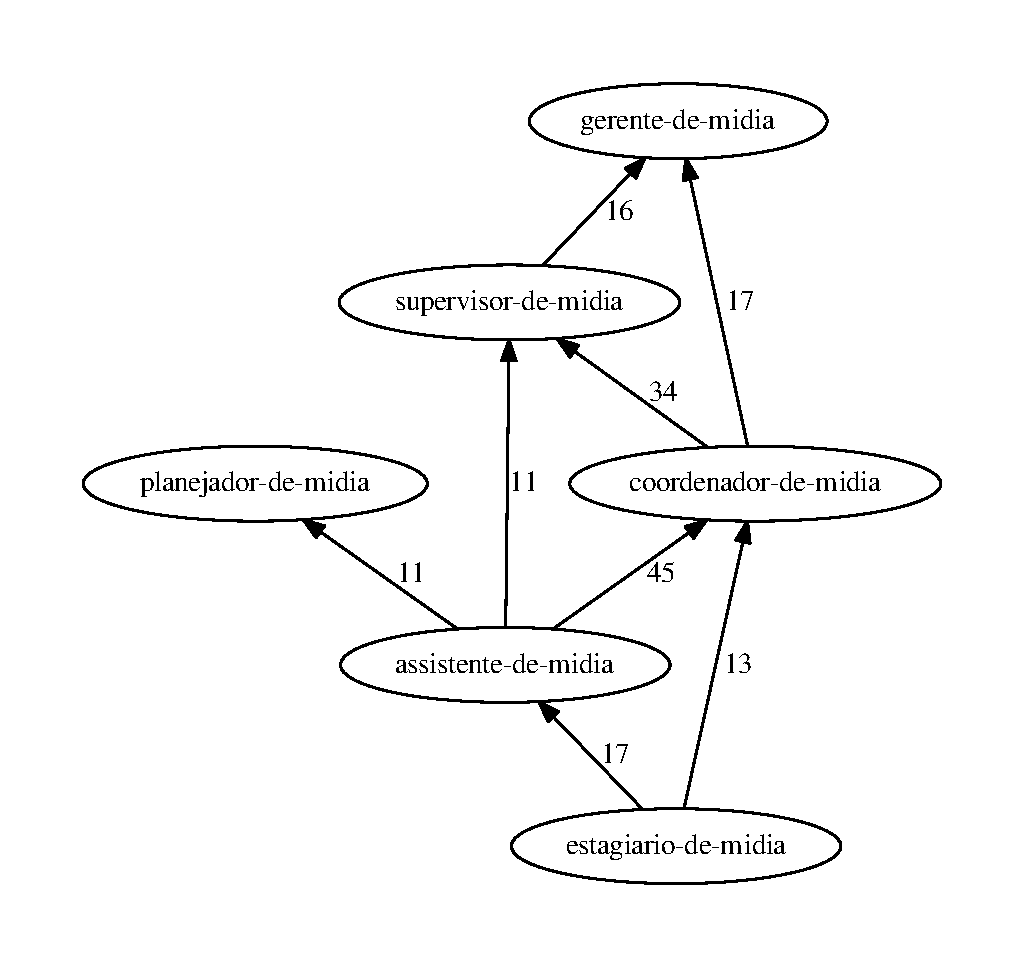
\includegraphics[scale=0.6]{cluster_23.pdf}
  \caption{Parte do MCar com ocupações relacionadas à carreira de mídia.}
  \label{fig:ex-mapa-midia}
\end{figure}

As ocupações no MCar foram definidas a partir de \textit{consenso} nos currículos. Como o título da ocupação é um campo em que o usuário digita livremente, assumiu-se que, se um grupo \enquote{suficientemente grande} de pessoas entra em acordo sobre uma certa nomenclatura, ela representa objetivamente uma ocupação. Essa abordagem é colocada de maneira implícita em ~\citeonline{Abbott1995-ft}, já \citeonline{Gunz2007-hr} a exploram para definir fronteiras de carreiras.

Uma das maiores dificuldades está em se definir o quanto um consenso precisa ser \enquote{suficientemente grande} para de fato existir uma ocupação. Para os fins desse trabalho, esse número foi obtido de forma experimental e empírica. Para isso, procurou-se o número mínimo de repetições exatas na grafia das ocupações de maneira que não fossem encontrados erros de digitação recorrentes, ou seja, que das ocupações criadas por consenso, nenhuma fosse resultado de erros frequentes de digitação. Esse número foi definido em 30 repetições, ou 10 transições com exatamente a mesma grafia em ambos os lados da transição.

Para a criação do MCar foram usados os currículos anonimizados de 10 milhões de usuários registrados no site VAGAS.com.br. A seleção de dados, bem como o processamento das informações, seguiu um procedimento conservador. Isso significa que as decisões tomadas em sua construção procuram minimizar os erros decorrentes da qualidade dos dados, mesmo que isso signifique trabalhar com uma quantidade menor deles. Utilizando o exemplo na Figura~\ref{fig:ex-mapa-midia}, isso significa que, provavelmente, muito mais do que 16 pessoas na base de dados fizeram a transição de \enquote{supervisor-de-midia} para a ocupação \enquote{gerente-de-midia}, porém, esses 16 são livres de erros e de subjetividade.

Da massa de currículos, apenas os atualizados no período entre 2011 e 2016 foram usados. Currículos em duplicação foram removidos usando o CPF como identificador; em caso de duplicação, apenas o currículo mais recente foi considerado. Na impossibilidade de se verificar a duplicação, como por exemplo, na ausência do CPF, o currículo também foi descartado.

Finalmente, algumas informações gerais foram extraídas dos currículos que passaram pelo processo acima e o restante das informações foi descartada, incluindo quaisquer maneiras de se identificar a pessoa descrita no currículo, garantindo a anonimidade do processo.

As informações extraídas são o sexo, último salário, graduação (se existente) ou escolaridade, e a sequência de ocupações pela qual o profissional passou com o título, descrição e período em que exerceu a ocupação.

O título da ocupação é um dos principais artefatos do MCar, é ele quem fornece a identidade para o nó. Como descrito acima, nos currículos, o título da ocupação é um campo de texto livre, ou seja, o usuário pode digitar o título sem restrições. Se por um lado isso permite a identificação de ocupações de nicho, novas ou que usem jargão de área; por outro isso significa que os títulos possuem erros de grafia, variações de gênero (como em \enquote{advogado} e \enquote{advogada} ou \enquote{moto boy} e \enquote{moto girl}), composição de múltiplas ocupações em um mesmo título (como \enquote{caixa/balconista}), abreviações e toda a gama de erros de interpretação possíveis.

As ocupações passam por um corretor ortográfico criado especificamente para esse trabalho, uma vez que um corretor tradicional não é capaz de identificar jargões de área como \enquote{enfermeiranda}, \enquote{rigger} ou \enquote{IRLA}.

Como exemplo, o dicionário do corretor possui cerca de 750 variações ortográficas que são traduzidas para o termo \enquote{auxiliar}, dentre eles, simples erros de omissão como \enquote{uxiliar}, até variações mais elaboradas como \enquote{ausciliar} e \enquote{alsilia}.

Após o trabalho de correção ortográfica, os títulos foram agrupados e contados. Especialistas da empresa verificaram os resultados dos maiores grupos para identificar anomalias, como ocupações com os títulos \enquote{sim}, \enquote{não} e \enquote{o mesmo}. Ocupações como essas foram excluídas do trabalho.

Finalmente, pares de ocupações foram gerados. Por exemplo, um currículo com a sequência de ocupações \enquote{saladeiro} $\to$ \enquote{chapeiro} $\to$ \enquote{cozinheiro} gera os pares \enquote{saladeiro} $\to$ \enquote{chapeiro} e \enquote{chapeiro} $\to$ \enquote{cozinheiro}.

Os pares foram agrupados e sua contagem se torna o peso de cada conexão na rede final. Nesse ponto do processo, cerca de 23 milhões de experiências profissionais são agrupadas em exatamente 7.450 ocupações distintas.

Finalmente, os pares de ocupações foram conectados entre si e a rede final foi construída e armazenada em um banco de dados de grafo. Um sistema online\footnote{Disponível em \url{http://www.vagas.com.br/mapa-de-carreiras}} disponibiliza as informações publicamente. Apesar de gratuito e de consulta pública, os dados do Mapa VAGAS da Carreira não são de uso livre. A empresa gentilmente cedeu os dados ao pesquisador para esse trabalho.

%===================================
\section{Grafos e Detecção de Comunidades} \label{sec:comunidades}
%===================================

Uma \textit{comunidade} é um subgrafo com conexões mais \textit{coesas} entre seus nós do que com nós do restante do grafo. A palavra \enquote{coesão} aqui pode ser interpretada de várias maneiras. Para \citeonline{Ahn2010-uh,Evans2009-lq}, uma comunidade é definida quando o número de conexões internas do subgrafo é maior que o número de conexões que o conecta ao resto do grafo. Para \citeonline{Barabasi2016-rn,Newman2004-jg} a comunidade deve possuir uma densidade de conexões mais alta do que o esperado em uma rede aleatória equivalente. Para esses autores, o número de conexões é o fator determinante para a identificação da comunidade.

\citeonline{Rosvall2009-sd,Van_Dongen2000-qm}, por sua vez, trabalham a detecção de comunidades como a identificação de fluxos mais frequentes na rede. Assumindo que uma conexão representa um fluxo, comunidades possuem fluxo maior entre seus nós do que com nós fora da comunidade.

Essas abordagens distintas são aplicáveis a cenários diferentes. A densidade de conexões é mais adequada em redes onde a estrutura é importante, como, por exemplo, em uma rede social. Já em redes que representam fluxos, como circuitos ou redes de transporte, a segunda abordagem é mais atraente~\cite{Rosvall2009-sd}.

Para esse trabalho, a identificação de comunidades por fluxo é adequada por concepção. Como exposto na Seção~\ref{sec:carreira}, as fronteiras de carreira são definidas pelo consenso das movimentações profissionais: transições menos frequentes definem essas fronteiras.

Essa frequência é relativa ao fluxo entre os nós próximos: dez transições para uma ocupação como \enquote{Auxiliar Administrativo}, que possui dezenas de milhares de profissionais entrando e saindo, não tem a mesma importância que para \enquote{Assistente de Mídia} (Figura~\ref{fig:ex-mapa-midia}), em que essa dezena representa mais de 10\% das transições registradas.

O algoritmo Infomap (detalhado na Seção~\ref{sec:infomap}) utiliza \textit{random walkers} para identificar comunidades. Os caminhos em que eles circulam mais frequentemente são considerados como fazendo parte da mesma comunidade; por outro lado, caminhos raramente utilizados definem as fronteiras entre uma comunidade e outra, de maneira análoga à concepção de fronteiras de carreira de~\citeonline{Gunz2007-hr}.

Portanto, por analogia, a identificação de comunidades do algoritmo Infomap identifica fronteiras de carreiras em uma rede em que as conexões representam o fluxo de profissionais entre ocupações, como é o caso do MCar.

Nesse trabalho, as comunidades são chamadas \textit{ilhas ocupacionais}.

%===================================
\subsection{O Algoritmo Infomap} \label{sec:infomap}
%===================================

Segundo \citeonline{Grunwald2007-bt}, quaisquer regularidades em um conjunto de dados podem ser usadas para comprimi-los, ou seja, descrevê-los usando uma quantidade menor de símbolos. Quanto maior a regularidade, maior a compressão, dessa forma, dentre várias representações possíveis dos dados, a que apresentar maior compressão é também aquela que melhor identifica padrões nos dados. A Descrição de Comprimento Mínimo (\textit{Minimum Description Length}) é a disciplina que estuda essa relação~\cite{Grunwald2007-bt}.

O algoritmo Infomap aproveita essa dualidade entre detecção de padrões e compressão de dados para identificar padrões de fluxo em redes~\cite{Rosvall2009-sd}.

Para compreender o algoritmo, é preciso entender como um trajeto aleatório em uma rede é representado e como a Descrição de Comprimento Mínimo usa essa representação na detecção de comunidades.

Para isso, descreve-se o caminho que um \textit{random walker} faz em uma rede através da sequência de nós pela qual ele passa. Por exemplo, assumindo uma rede com os nós $A$, $B$ e $C$, um caminho possível poderia ser descrito por $ABACBA$.

A Figura~\ref{fig:graph01} mostra um grafo regular, onde todos os nós possuem três vizinhos. Nesse tipo de rede, um \textit{random walker} ergódico (de caminho infinito) percorre todas as conexões o mesmo número de vezes. A Figura~\ref{fig:walk01} mostra um caminho aleatório passando por 800 nós.

\begin{figure}[ht]
  \centering
  \subfloat[][Rede regular] {
    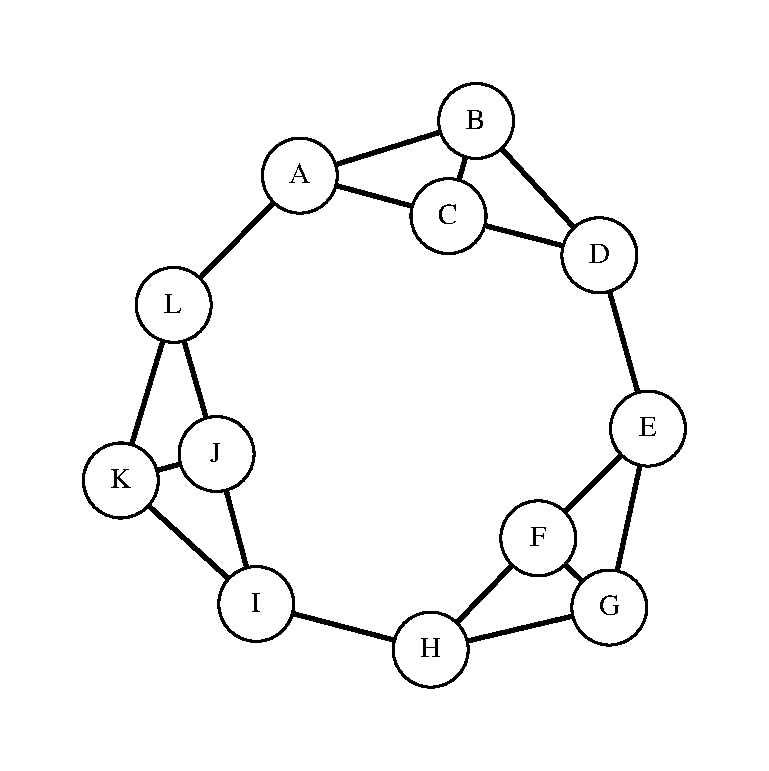
\includegraphics[scale=0.4]{graph01.pdf}
    \label{fig:graph01}
  }
  \subfloat[][Caminho na rede] {
    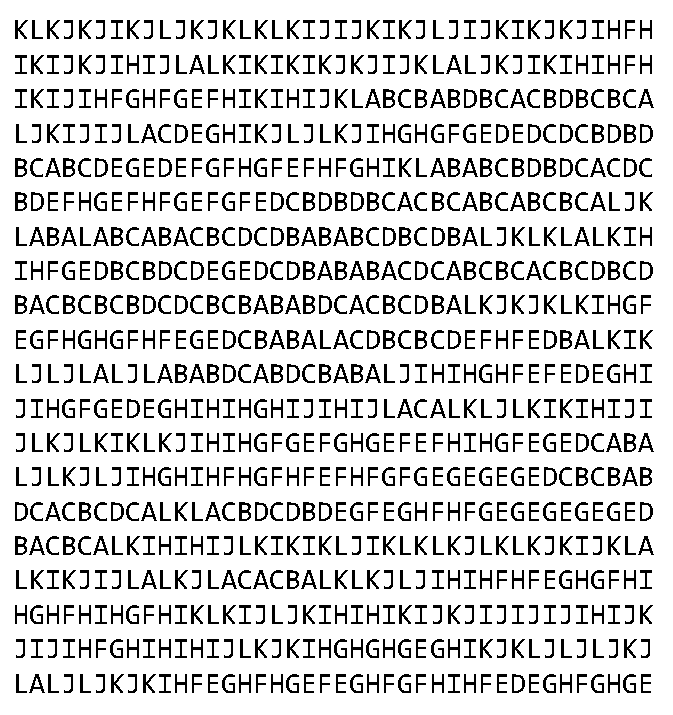
\includegraphics[scale=0.4]{graph01_path.pdf}
    \label{fig:walk01}
  }    
  \caption{Caminho de um \textit{random walker}}
\end{figure}

Apesar de ser uma rede regular, onde cada nó possui três conexões, sua topologia faz com que o \textit{random walker} fique \enquote{preso} nos grupos formados pelos nós $ABCD$, $EFGH$ e $IJKL$; escapando esporadicamente de um para outro, onde circula até escapar novamente. Esses grupos são destacados na Figura~\ref{fig:graph02}. O caminho percorrido pelo \textit{walker} é exibido na Figura~\ref{fig:walk02}, dessa vez destacando os grupos por onde ele passa. As cores em ambas as figuras torna fácil perceber seu comportamento.

\begin{figure}[ht]
  \centering
  \subfloat[][Rede regular] {
    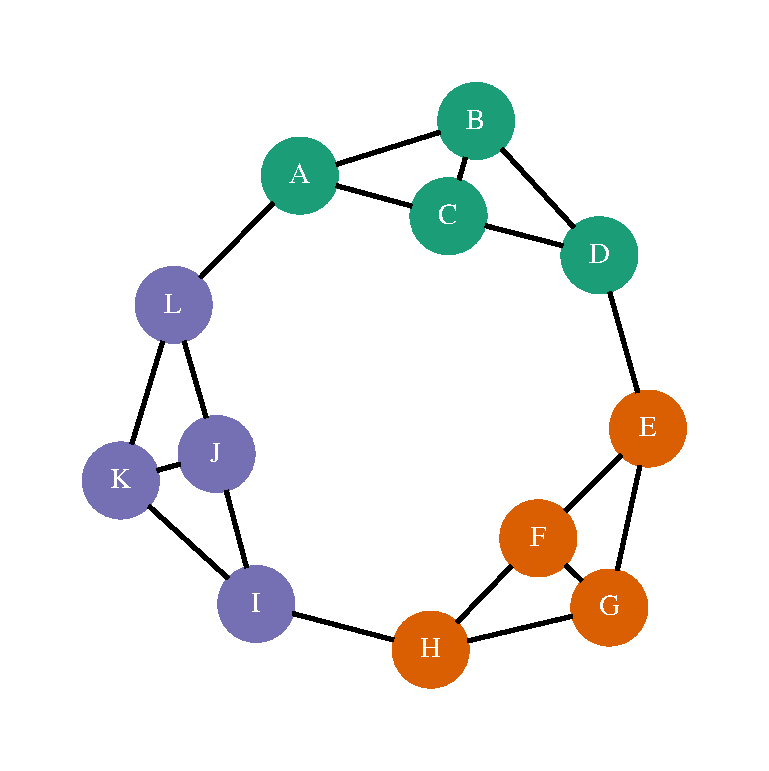
\includegraphics[width=0.4\linewidth]{graph02.pdf}
    \label{fig:graph02}
  }
  \subfloat[][Caminho na rede] {
    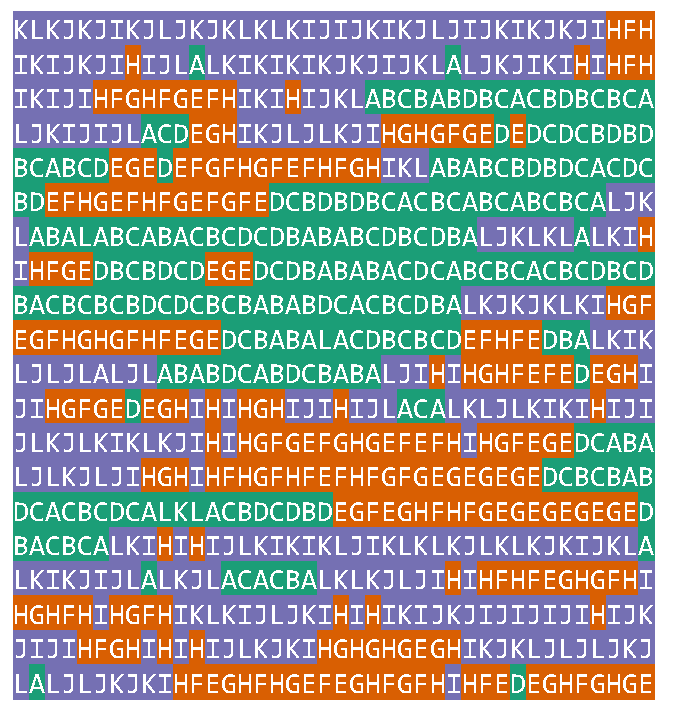
\includegraphics[width=0.4\linewidth]{graph02_path.pdf}
    \label{fig:walk02}
  }    
  \caption{Rede e caminho destacados}
\end{figure}

Se cada nó for representado por uma sequência de bits, podemos medir quanta informação é necessária para representar o caminho feito pelo \textit{random walker}. Usando a codificação de tamanho variável de  \citeonline{Huffman1952-ak} os nós mais frequentes são representados por códigos menores, resultando em uma codificação menor para representar um caminho do que uma que use códigos de tamanho fixo.

Os códigos usados por cada grupo são chamados \textit{codebooks}, os códigos que indicam qual \textit{codebook} será usado também é um \textit{codebook}, funcionando como um índice. Na Figura~\ref{fig:graph04}, existem três deles, um para cada grupo, contendo os nós \enquote{00}, \enquote{01}, \enquote{10}, \enquote{110} e o código de saída \enquote{111}. O \textit{codebook} índice possui os códigos: \enquote{0}, \enquote{10} e \enquote{11}.

Dessa forma o caminho que começa no nó mais abaixo do grafo da Figura~\ref{fig:graph03} e termina no nó do canto superior esquerdo é descrito pela sequência binária \enquote{000 1110 1011 1111 1101}, usando 19 bits. O mesmo caminho, usando a codificação da Figura~\ref{fig:graph04} é \enquote{\textbf{0} 01 110 \textit{111} \textbf{11} 00 01 10} possui 17 bits, onde os números em negrito indicam entrada em um grupo e o número em itálico indica saída do grupo.

Nesse caminho curto, ambas as codificações têm tamanhos similares, Porém, em um caminho infinitamente longo (ergódico), o uso de múltiplos \textit{codebooks} pode produzir um código mais compacto do que o uso de um único \textit{codebook}. Como exemplo, o caminho da Figura~\ref{fig:walk01} usando a codificação da Figura~\ref{fig:graph03} possui 2880 bits, enquanto possui 1776 bits usando a codificação da Figura~\ref{fig:graph04}.

\begin{figure}[ht]
  \centering
  \subfloat[][Nós usando codificação de Huffman] {
    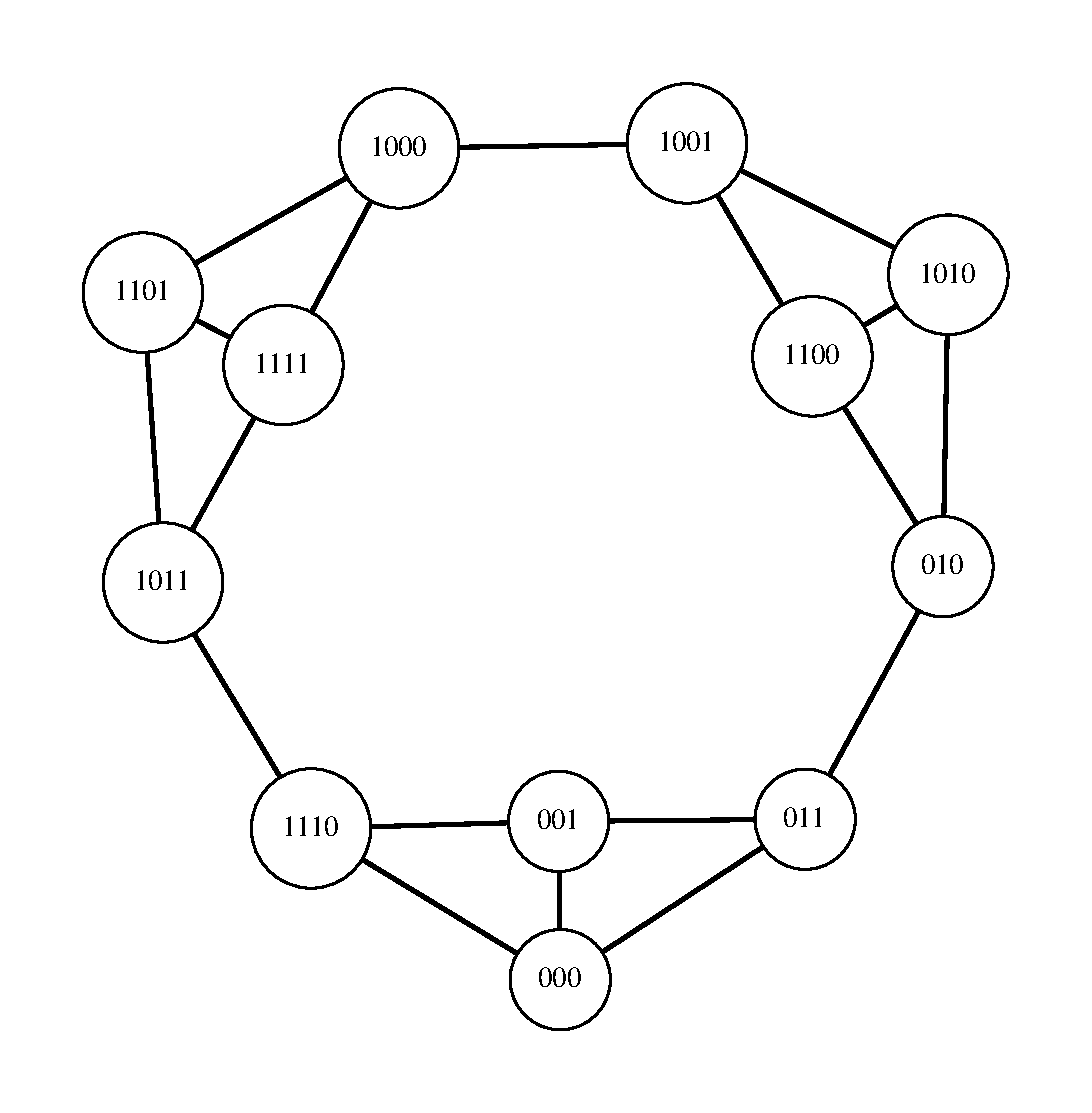
\includegraphics[width=0.4\linewidth]{graph03.pdf}
    \label{fig:graph03}
  }
  \subfloat[][Reaproveitamento de códigos] {
    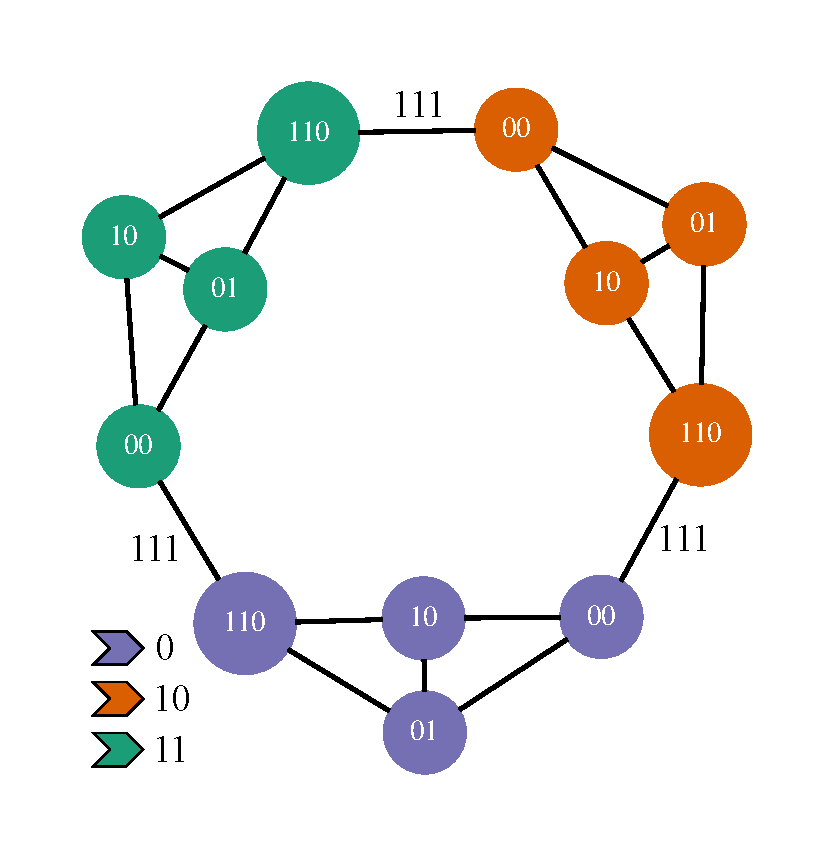
\includegraphics[width=0.4\linewidth]{graph04.pdf}
    \label{fig:graph04}
  }    
  \caption{Codificação dos nós}
\end{figure}

O particionamento da rede em grupos onde os caminhos aleatórios podem ser representados da maneira mais compacta possível deve representar o melhor particionamento em relação ao fluxo.

A \enquote{Equação de Mapa}\footnote{No original: \textit{Map Equation}}~\cite{Rosvall2009-sd} permite que se identifiquem as menores codificações possíveis para um determinado particionamento da rede sem a necessidade de se empregar \textit{random walkers} de fato. Com ela, a detecção de comunidades usando o fluxo como critério de coesão se reduz a um problema de otimização.

A Equação de Mapa é
\begin{equation} \label{eq:map-equation}
  L(\mathsf{M}) = q_\curvearrowright H(\mathcal{Q}) + \sum_{i=1}^{m}p^i_\circlearrowright H(\mathcal{P}^i)\,,
\end{equation}
onde $L(\cdot)$ é o menor tamanho de codificação possível para representar um certo particionamento; $\mathsf{M}$ é o particionamento dos nós em $m$ comunidades; $i = 1, 2, \ldots, m$; $q_\curvearrowright$ é a probabilidade de um \textit{random walker} sair de qualquer comunidade e passar para o \textit{codebook} índice; $H(\mathcal{Q})$ (\textit{eta} em maiúsculo) é número médio de bits usado para representar o \textit{codebook} índice segundo a distribuição de probabilidade $\mathcal{Q}$; e $H(\mathcal{P}^i)$ também é o número médio de bits, mas dessa vez daqueles usados na comunidade $i$ segundo a distribuição $\mathcal{P}^i$; finalmente $p^i_\circlearrowright$ é a probabilidade do \textit{walker} estar na comunidade $i$.

$H(\textbf{p})$ é a equação que descreve a entropia da informação segundo uma certa distribuição de probabilidade $\textbf{p}$~\cite{Shannon1948-ic}. Ela se refere a média de bits necessária, por símbolo, para se representar a informação gerada por um processo estocástico e é expressa como:
\begin{equation*}
H(\textbf{p}) = - \sum_\alpha p_\alpha \log_2 p_\alpha\,.
\end{equation*}

Nessa equação, $p_\alpha$ é a probabilidade estacionária do \textit{walker} passar pelo nó$\alpha$, ou seja, em um caminho infinito, qual fração de tempo o \textit{walker} teria passado por $\alpha$~\cite{Rosvall2009-sd}.

Para calcular $p_\alpha$ inicia-se com a matriz estocástica linear $W$, gerada a partir da matriz de adjacência $A$ direcionada e ponderada. Em uma matriz estocástica linear, a soma dos pesos de entrada do nó (linha) é normalizado para que resulte em 1. Cada elemento $w_{\alpha \beta}$ dessa matriz representa a probabilidade de um \textit{random walker}  em $\alpha$ chegar ao nó $\beta$.  Transportada para a realidade do MCar, essa é a probabilidade de alguém na ocupação $\alpha$ fazer a transição para a ocupação $\beta$.

Sendo $n$ o número de nós da rede, define-se $w_{\alpha \beta}$ como:
\begin{align} \label{eq:matriz-estocastica}
w_{\alpha \beta} = 
    \begin{cases*}
        \frac{1}{n}, & \text{se $\alpha$ não possui conexões de saída, ou seja, $\sum_\beta A_{\alpha \beta} = 0$,} \\
        0, & \text{se não há conexão entre $\alpha$ e $\beta$,} \\
        \frac{A_{\alpha \beta}}{\sum_\beta A_{\alpha \beta}}, & \text{caso contrário.}
    \end{cases*}
\end{align}

A primeira cláusula da Equação~\ref{eq:matriz-estocastica} garante que a matriz estocástica possua linhas totalizando 1 quando o nó não possui conexões de saída. Para efeitos do \textit{random walker}, isso significa que ele se teleporta para um nó qualquer da rede quando se encontra em um nó sem saída. Caso contrário, os nós sem conexões de saída acumulariam a probabilidade total da rede~\cite{Franceschet2011-ef}.

A probabilidade estacionária $p_\alpha$ é calculada pelo sistema de equações
\begin{equation} \label{eq:page-rank}
p_\alpha = \sum_\beta (1 - \tau) p_\beta w_{\beta \alpha} + \frac{1}{n} \tau\,,
\end{equation}
onde $\tau$ é a probabilidade do \textit{walker} ser teleportado para um nó aleatório. A primeira cláusula da Equação~\ref{eq:matriz-estocastica} e a presença de $\tau$ transformam o \textit{random walker} em um \textit{random surfer}. Esse artifício foi usado por~\citeonline{Page1999-ag} na criação do algoritmo de PageRank e fornece a base para a Equação de Mapa.

O recurso de teleporte garante a ergodicidade do caminho e, segundo o teorema de Perron-Frobenius, faz com que a probabilidade estacionária seja definida~\cite{Rosvall2009-sd}.

A partir de $p_\alpha$, é possível expandir a Equação de Mapa.

Sendo $q_{i \curvearrowright}$ a probabilidade de saída da comunidade $i$, $q_{\curvearrowright}$ é a probabilidade de saída de qualquer comunidade. O valor de $q_{\curvearrowright}$ equivale à taxa de uso do \textit{codebook} índice, uma vez que a saída de uma comunidade implica  em seu uso para indicar qual a próxima comunidade.

Finalmente, sendo $n$ o número de nós da rede e $n_i$ o número de nós pertencente à comunidade $i$, expande-se a Equação~\ref{eq:map-equation} em
\begin{align}
q_{i \curvearrowright} &= \tau \frac{n - n_i}{n} \sum_{\alpha \in i} p_\alpha + (1 - \tau) \sum_{\alpha \in i} \sum_{\beta \nin i} p_\alpha w_{\alpha \beta} \nonumber \\
q_\curvearrowright       &= \sum_{i = 1}^m q_{i\curvearrowright} \nonumber \\
p^i_\circlearrowright    &= q_{i \curvearrowright} + \sum_{\alpha \in i} p_\alpha \nonumber \\
H(\mathcal{Q})            &= - \sum_{i = 1}^m \frac{q_{i \curvearrowright}}{q_\curvearrowright} \log_2 \frac{q_{i \curvearrowright}}{q_\curvearrowright} \nonumber \\
H(\mathcal{P}^i)         &= - \frac{q_{i \curvearrowright}}{p^i_\circlearrowright} \log_2 \frac{q_{i \curvearrowright}}{p^i_\circlearrowright} 
-  \sum_{\alpha \in i} \frac{p_\alpha}{p^i_\circlearrowright} \log_2  \frac{p_\alpha}{p^i_\circlearrowright} \nonumber \\
L(\mathsf{M})              &= q_\curvearrowright \log_2 q_\curvearrowright - 2 \sum_{i = 1}^m q_{i \curvearrowright} \log_2 q_{i \curvearrowright} - \sum_{\alpha = 1}^n p_\alpha \log_2 p_\alpha + \sum_{i = 1}^m p^i_\circlearrowright \log_2 p^i_\circlearrowright\,.
\end{align}

Existem variações da Equação de Mapa para detecção de comunidades sobrepostas~\cite{Viamontes_Esquivel2011-it} e hierárquicas~\cite{Rosvall2011-yi}. Este trabalho usa ambas as variações.

Para o algoritmo que permite que os nós pertençam a mais de uma comunidade, \citeonline{Viamontes_Esquivel2011-it} usam \textit{conexões com memória} para lembrar o passo anterior do \textit{random walker}. No caso de se mover para um nó que pertence à múltiplas comunidades, ele se manterá na comunidade de onde veio, se possível.

Para isso, duas alterações são feitas na Equação de Mapa: mudança da definição de $p_\alpha$ para considerar nós em múltiplas comunidades (detalhada na Equação~\ref{eq:page-rank-overlap}) e a soma das probabilidades condicionais desses nós (detalhada mais à frente na Equação~\ref{eq:map-equation-overlap}).

Na equação original, a probabilidade estacionária $p_\alpha$ de um \textit{random walker} estar em um nó $\alpha$ é dada pelo Equação~\ref{eq:page-rank}. Na variação com sobreposição, cada nó $\alpha$ possui uma probabilidade separada de estar em uma comunidade $i$, a probabilidade estacionária $p_{\alpha_i}$ é resolvida pelo sistema de equações
\begin{equation} \label{eq:page-rank-overlap}
p_{\alpha_i} = \sum_\beta \sum_{j \in M_\beta} p_{\beta_j} \delta_{\alpha_i \beta_j} \left[ (1 - \tau)  w_{\beta \alpha} + \frac{1}{n} \tau \right],
\end{equation}
onde $\delta_{\alpha_i \beta_j}$ é a função de transição entre comunidades, definida como
\begin{equation*}
\delta_{\alpha_i \beta_j} =
    \begin{cases*}
    1,                              & \text{se $i = j$},\\
    \frac{1}{|M_\beta|} & \text{se $i \neq j$ e $i \notin M_\beta$},\\
    0,                              & \text{se $i \neq j$ e $i \in M_\beta$}.
    \end{cases*}
\end{equation*}

A Equação de Mapa para comunidades com sobreposição é
\begin{equation} \label{eq:map-equation-overlap}
    L(\mathsf{M}) = q_\curvearrowleft \log_2 q_\curvearrowleft
                               - 2 \sum_{i=1}^m q_{i \curvearrowright} \log_2 q_{i \curvearrowright}
                               - \sum_{i=1}^m \sum_{\alpha \in i} p_{\alpha_i} \log_2  p_{\alpha_i}
                               + \sum_{i=1}^m p^i_\circlearrowright \log_2 p^i_\circlearrowright\,.                            
\end{equation}

A variação hierárquica do algoritmo possibilita detecção de comunidades aninhadas, nesse caso, ela é uma generalização da Equação de Mapa original que permite que múltiplos \textit{codebooks}.

%% SE USAMOS AS VARIAÇÕES DA EQUAÇÃO DE MAPA, ENTÃO PRECISAMOS APRESENTÁ-LAS AQUI
% Ronie: Feito!!!! Demorou uma vida pra entender como as equações dos três artigos se relacionavam, mas entendi :) A pior parte foi entender que a matriz estocástica W é linear, enquanto que nos materiais introdutórios ela é _sempre_ colunar, essa confusão me fez ficar dois fins se semana batendo a cabeça com 'essa conta não faz sentido'. Pois é, não fazia mesmo.
% Ronie: Está faltando só a equação hierárquica, estou escrevendo ela agora.

%===================================
\section{Assortatividade} \label{sec:assortatividade}
%===================================

A assortatividade é uma medida de quão nós similares estão conectados entre si~\cite{Newman2003-jn}. Quaisquer atributos dos nós podem ser usados como medida de assortatividade, por exemplo, se nós representarem pessoas e as conexões representarem amizades, medir a assortatividade de idade diria se as pessoas preferem amizades com outras de idade similar (assortatividade positiva) ou preferem amizades com pessoas muito mais velhas ou novas (assortatividade negativa ou desassortatividade).

A assortatividade de grau é de especial interesse na análise de redes, pois permite caracterizar sua topologia. Redes com assortatividade negativa (desassortativas), remetem à topologia de \enquote{eixo e raios} (\textit{hub and spokes}), onde nós de grau muito alto (\textit{hubs}) se conectam a muitos nós de grau mais baixo~\cite{Barabasi2016-rn}. A Figura~\ref{fig:ex-sobreposicao-ti} mostra um exemplo de uma rede em que predomina essa topologia.

Quanto menor a assortatividade, mais a rede se aproxima da topologia de \enquote{estrela}, em que todos os nós de alto grau só se conectam a nós de grau muito baixo. Como exemplos, a ilha ocupacional relacionada a \enquote{fisioterapia} na Figura~\ref{fig:ex-fisioterapeutas}, com assortatividade $-0,27$, possui todos os nós conectados a um \textit{hub} central, com poucas conexões entre ocupações periféricas. Já a ilha relacionada a \enquote{bolsistas} na Figura~\ref{fig:ex-bolsistas}, com assortatividade $-0,07$, não possui um \textit{hub} tão claramente definido; ainda que existam alguns nós folhas conectados a nós de maior grau, boa parte dos nós possui grau similar.

\begin{figure}[ht]
    \centering
    \subfloat[][Assortatividade $-0,27$] {
        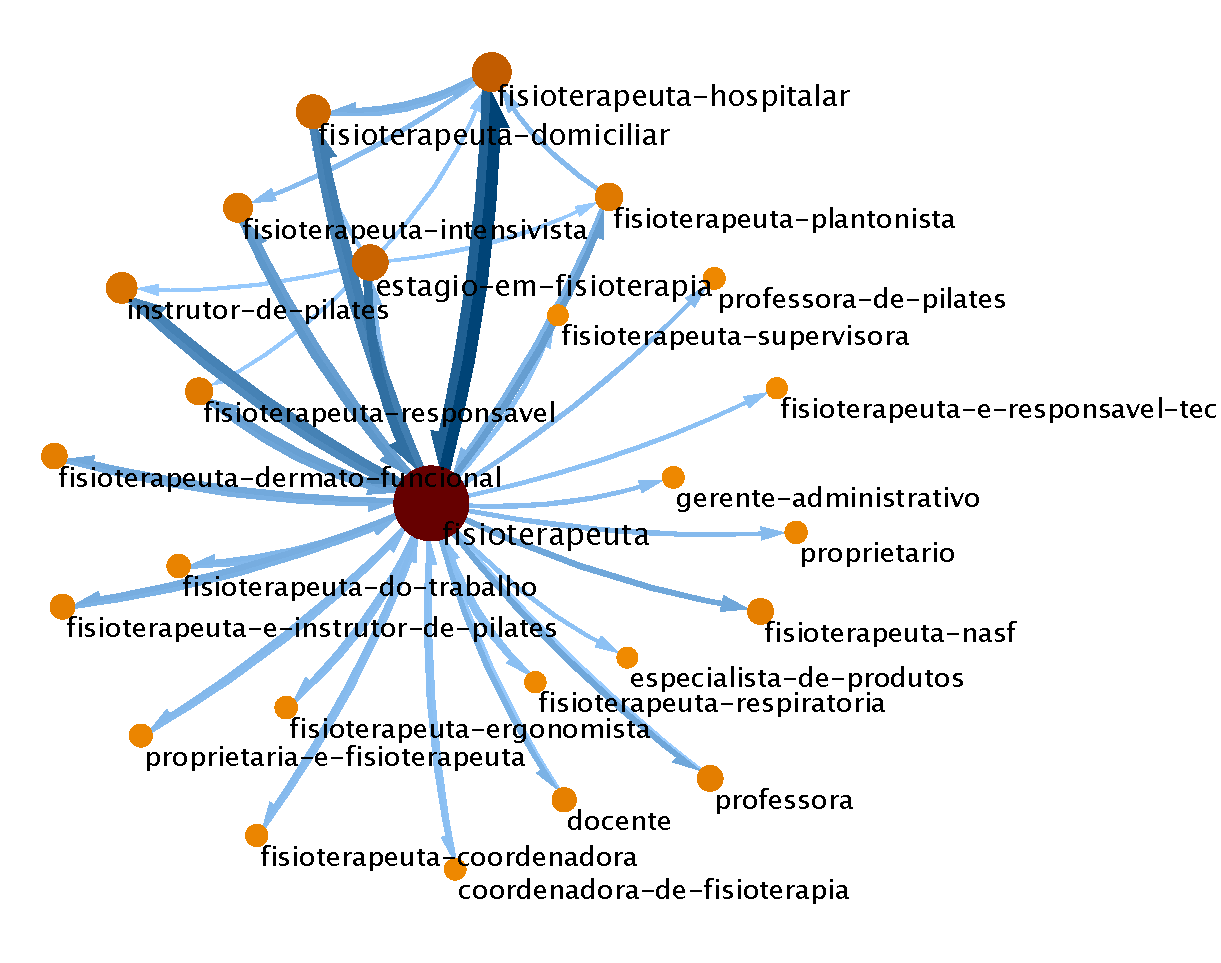
\includegraphics[width=0.4\linewidth]{ex-sobreposicao-fisioterapeutas.pdf}
        \label{fig:ex-fisioterapeutas}
    }
    \subfloat[][Assortatividade $-0,07$] {
        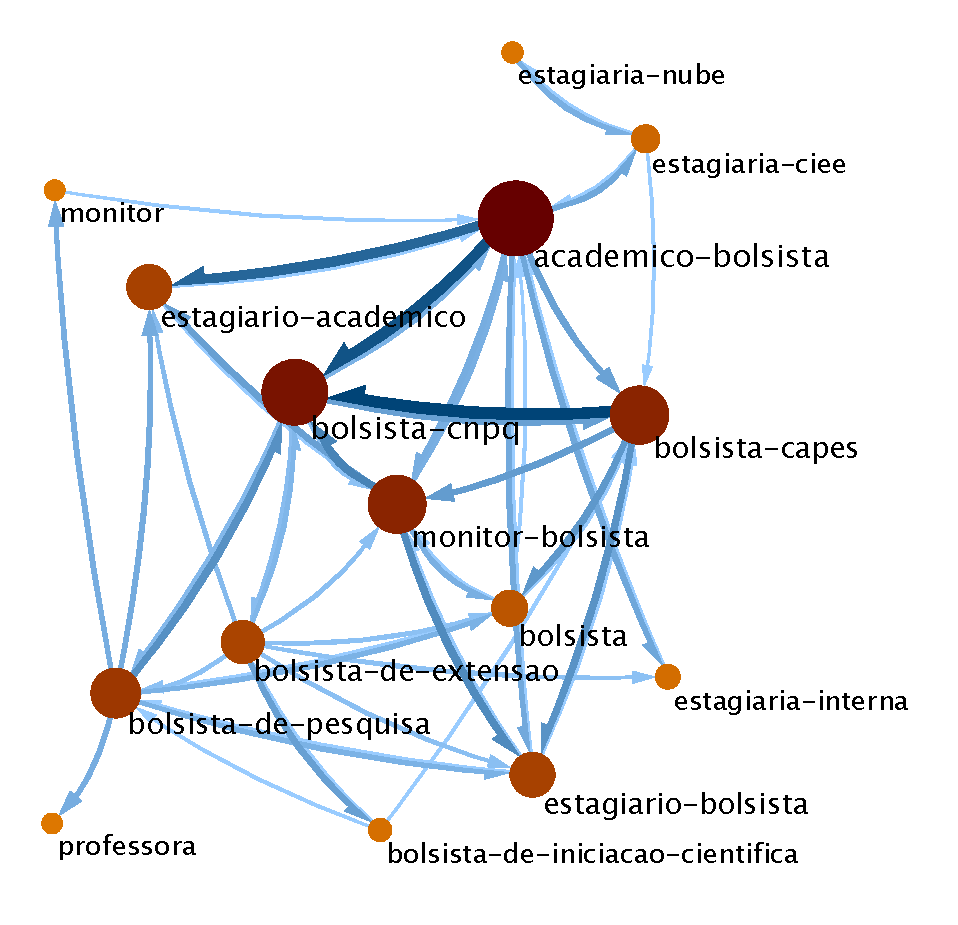
\includegraphics[width=0.4\linewidth]{ex-sobreposicao-bolsistas.pdf}
        \label{fig:ex-bolsistas}
    }    
    \caption{Assortatividade e Topologia}
\end{figure}

A assortatividade de grau em uma rede direcionada pode ser caracterizada pelo coeficiente de correlação de Pearson dos graus~\cite{Barabasi2016-rn}. Seja $k_i^\leftarrow$ e $k_i^\rightarrow$,  respectivamente, os graus de entrada e saída do nó $i$, $E$ o conjunto de conexões da rede, $e = (m, n) \mid e \in E$ as conexões de $E$, $m$ o vértice de onde $e$ sai e $n$ o vértice para onde $e$ aponta, definem-se os \textit{graus remanescentes} $\delta_e^\leftarrow$ e $\delta_e^\rightarrow$ da conexão $e$ como

\begin{align*}
\delta_e^\leftarrow &= k_n^\leftarrow - 1
\\
\delta_e^\rightarrow &= k_m^\rightarrow - 1\,.
\end{align*}

\begin{figure}[ht]
    \centering
    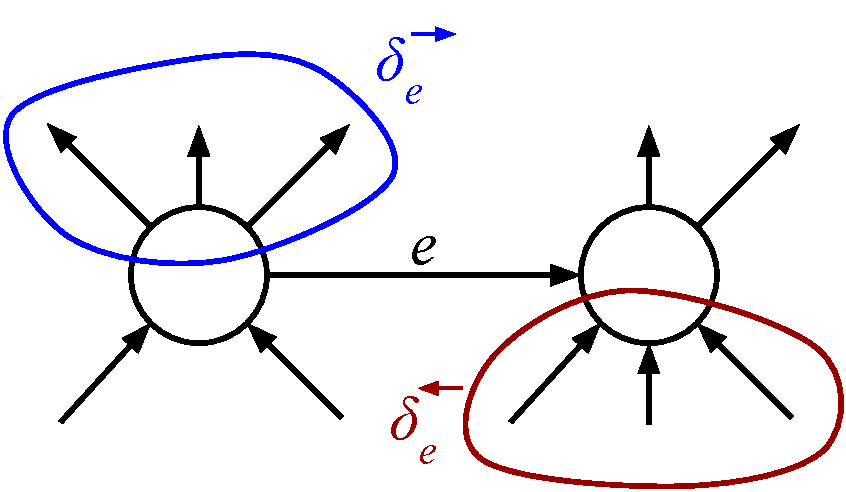
\includegraphics[scale=0.4]{remaining-degree.pdf}
    \caption{Graus remanescentes de entrada e saída da conexão $e$}
    \label{fig:remaining-degree}
\end{figure}

O \textit{grau remanescente} é o grau do nó, excetuando-se a conexão atual (Figura~\ref{fig:remaining-degree}). A correlação de Pearson $r$ dos graus é então definida por

\begin{align*}
p &= \sum_{e \in E} \delta_e^\leftarrow \delta_e^\rightarrow
\\
q &= \frac{1}{|E|} \sum_{e \in E} \delta_e^\leftarrow
                                  \sum_{e \in E }\delta_e^\rightarrow
\\
\sigma^2_\leftarrow &= \sum_{e \in E} \left( \delta_e^\leftarrow \right)^2
            - \frac{1}{|E|} \left( \sum_{e \in E} \delta_e^\leftarrow \right)^2
\\
\sigma^2_\rightarrow &= \sum_{e \in E} \left( \delta_e^\rightarrow \right)^2
           - \frac{1}{|E|} \left( \sum_{e \in E} \delta_e^\rightarrow \right)^2
\\
r &= \frac{p - q}
                {\sqrt{ \sigma^2_\leftarrow } \sqrt{ \sigma^2_\rightarrow }}\,.
\end{align*}


%===================================
\section{Resultados e Análises} \label{sec:resultados}
%===================================

% Descrição dos dados:

A versão do MCar usada nesse trabalho é de fevereiro de 2017. Ela possui exatamente 7.450 ocupações distintas e 90.800 conexões.

A rede de ocupações possui a distribuição de grau exibida no gráfico de Pareto da Figura~\ref{fig:pareto-grau}. Ela possui uma grande concentração de conexões em poucos nós, formando \textit{hubs}. Os 25,01\% nós de maior grau são responsáveis por 88,76\% das conexões da rede.

Por ser uma rede direcionada, um certo cuidado na análise é necessário, uma vez que o grau dos nós não corresponde diretamente ao número de nós conectados. Imaginando que cada nó pode uma ou duas conexões com um nó vizinho, o grau $k_i$, varia em relação ao número de vizinhos entre $k_i = v_i$ e $k_i = 2v_i$, onde $v$ é o número de nós conectados ao nó $i$ por uma conexão de entrada ou saída.

O quanto cada nó contribui para a conectividade da rede pode ser observada no gráfico de Pareto da Figura~\ref{fig:pareto-subgrafo}. As ocupações estão ordenadas pelo número de nós no subgrafo formado pela ocupação e todos os seu nós vizinhos. Exatamente 10\% dos nós com mais vizinhos são suficientes para conectar 95,77\% da rede.

O nó de maior grau \textit{Auxiliar Administrativo} possui 6.308 das 90.800 conexões da rede, mas forma um subgrafo com os nós vizinhos com 3.962 dos 7.450 nós da rede, ou seja, 53,18\% das ocupações de alguma forma possui fluxo de profissionais saindo ou entrando dessa ocupação.

Na Figura~\ref{fig:pareto-subgrafo}, o acumulativo considera apenas o nós \textit{novos} em relação às ocupações anteriores. Por exemplo, a segunda ocupação mais conectada (\textit{Vendedor}, com 2215 nós vizinhos) possui apenas 218 nós \enquote{inéditos} em relação a \textit{Auxiliar Administrativo}, a terceira ocupação (\textit{Assistente Administrativo}, com 2.192 nós vizinhos) contribui apenas com 83 nós não conectados pelas duas ocupações anteriores.

%% AH, VOCÊ NÃO VAI DEIXAR O LEITOR CURIOSO PARA SABER QUAL É ESSA OCUPAÇÃO QUE SE CONECTA COM QUASE TODAS AS OUTRAS, VAI? DIZ AÍ! E ESCREVA TAMBÉM. INCLUSIVE, VALEM ALGUNS COMENTÁRIOS SOBRE TAL OCUPAÇÃO.

%Ronie: Fiz uma besteira aqui, esqueci de tirar a conexões duplicadas (ida e volta) para gerar o número que estava antes. Quando fui conferir, percebi o erro. Acabou que revisei todos os números e gráficos, por medo.

\begin{figure}[htb]
  \centering
  \subfloat[][Pareto por Grau] {
    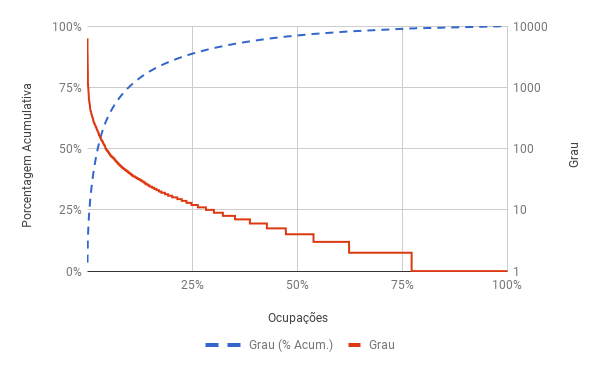
\includegraphics[width=0.49\linewidth]{pareto-grau}
    \label{fig:pareto-grau}
  }    
  \subfloat[][Pareto por Subgrafo Conectado] {
      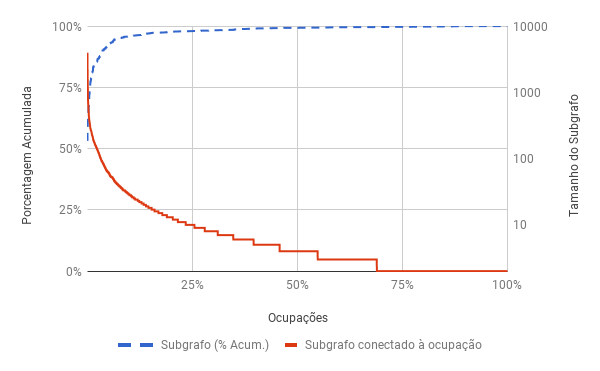
\includegraphics[width=0.49\linewidth]{pareto-subgrafo}
      \label{fig:pareto-subgrafo}
  }  
  \caption{Gráficos de Pareto com a distribuição de grau  do MCar e com o tamanho dos subgrafos formados pelos nós com maior conectividade. Os gráficos estão colocados lado a lado para facilitar a comparação. Os nós estão ordenados de maneira decrescente no eixo horizontal; na Figura~\ref{fig:pareto-grau}  as ocupações de grau maior no estão à esquerda e ocupações de menor grau estão à direita. na Figura~\ref{fig:pareto-subgrafo} elas estão ordenadas pelo tamanho do subgrafo formado pela ocupação e todos os seus vizinhos. Os eixos direitos, em escala logarítmica, estão associados às linhas cheias e representam, respectivamente, o grau do nó e o tamanho do subgrafo. Os eixos esquerdos estão associados às linhas tracejadas; na Figura~\ref{fig:pareto-grau} ela representa a somatória de todos os graus em porcentagem e qual a contribuição das ocupações à esquerda para essa totalização; na Figura~\ref{fig:pareto-subgrafo} ela representa a quantidade de ocupações que o subgrafo formado pelas ocupações à esquerda}
  \label{fig:paretos}
\end{figure}

Observando a Figura~\ref{fig:paretos} é possível notar que quase $1/4$ das ocupações possui apenas uma conexão (1.689 delas, 22,67\%), mas pouco menos de $1/3$ (2.317 delas, 31,10\%) possui apenas um nó vizinho.

Essa característica parece reforçar o conceitos sobre movimentação profissional como a Carreira sem Fronteiras e a Carreira Proteana, indicando que uma grande quantidade de profissionais trilha por carreiras variadas e se adaptam a diferentes ocupações. No entanto, há uma rápida queda no número de conexões, sugerindo que esses conceitos não se aplicam a todas as ocupações igualmente. O \enquote{Paradoxo da Amizade}~\cite{Barabasi2016-rn} parece valer para pessoas transitando entre ocupações. O paradoxo é dado como \enquote{na média, meus amigos são mais populares que eu}, transportado para o contexto desse trabalho seria enunciado como \enquote{na média, os outros trabalhos que eu poderia executar têm mais opções de movimentação que o meu}. Esse paradoxo tem uma explicação simples, como se observa na Figura~\ref){fig:pareto-subgrafo}, um nó qualquer têm grandes chances de estar conectado a um ou mais \textit{hubs} o que, na média, faz com que as ocupações vizinhas tenham mais conexões do que as suas próprias.

%% NA CIÊNCIA PRECISAMOS SER EXATOS. NÃO PODEMOS FICAR USANDO APROXIMADAMENTE O TEMPO TODO, OK? PADRONIZE DUAS CASAS DECIMAIS PARA PERCENTUAIS E ARREDONDE OS INTEIROS SE NECESSÁRIO.
% Ronie: Okay!

% Procedimento:

Nos experimentos realizados, o algoritmo Infomap foi utilizado para encontrar o particionamento mais coeso do MCar em relação ao fluxo. Como exposto nas Seções~\ref{sec:carreira} e~\ref{sec:infomap}, esse particionamento é a própria definição de fronteiras de carreira.

O Infomap é bastante robusto quanto aos parâmetros utilizados, ou seja, mesmo grandes variações em seus parâmetros devem produzir resultados similares~\cite{Kawamoto2015-ha,Lambiotte2012-fp}. Por essa razão e para comparação com o trabalho de \citeonline{Viamontes_Esquivel2011-it}  os parâmetros padrões foram utilizados: a probabilidade de teleporte para uma conexão aleatória de 0,15 e tempo de Markov em 1.

Para esse algoritmo, quanto maior a compressão da informação do caminho do \textit{random walker}, melhor é o particionamento da rede~\cite{Rosvall2009-sd}.

O MCar foi testado em três variações do algoritmo: 
\begin{itemize}
\item Simples: consiste na detecção de comunidades em que cada nó pertence a apenas uma única comunidade. 
\item Hierárquica: detectam-se comunidades dentro de outras. 
\item Com sobreposição: permite-se que nós participem de mais de uma comunidade.
\end{itemize}

A variação com maior compressão revela a melhor caracterização de particionamento~\cite{Viamontes_Esquivel2011-it,Rosvall2011-yi}. Se uma rede possuir maior compressão de informação com a variação hierárquica do que com a variação simples, assume-se que ela inerentemente possui uma estrutura de comunidades aninhadas. Se a variação com sobreposição possuir maior compressão de informação do que as outras, assume-se que suas comunidades, intrinsecamente, compartilham nós.

Os resultados de compressão para cada variação são apresentados na Tabela~\ref{tab:metodos}. É possível observar que as variações simples e hierárquica possuem quase a mesma compressão (os valores na tabela são aproximados), isso significa que o MCar não possui uma organização inerentemente hierárquica. Por outro lado, há um ganho expressivo de compressão de informação quando se permite a sobreposição de comunidades, revelando que existem ocupações compartilhadas entre grupos profissionais diferentes. Ainda assim, uma quantidade relativamente pequena de ocupações, cerca de 11\%, é compartilhada entre ilhas.

% INTUITIVAMENTE UMA COMPRESSÃO MAIOR IMPLICA EM MENOS COMUNIDADES, PORÉM SUA TABELA MOSTRA O CONTRÁRIO, ASSIM COMO O TEXTO. DE ACORDO COM SUA EXPLICAÇÃO UMA MAIOR COMPRESSÃO IMPLICA EM MELHOR PARTICIONAMENTO E, PORTANTO, MAIS COMUNIDADES.
% Ronie: Aqui acho que preciso melhorar a explicação. Como tb não expliquei as variações hierárquicas e com sobreposição do Infomap estão também falta uma peça do quebra cabeças. A compressão dessa 'descrição do caminho do random walker' acaba criando um balanço entre quantidade de nós e de comunidades. Se não houverem 'gargalos' de fluxo, o random walker não fica 'preso' em um subgrafo e a melhor compressão acontece simplesmente por códigos mais curtos nos nós mais frequentes, sem divisão em comunidades. Por outro lado, quando existe um gargalo o random walker fica preso por um longo tempo de um lado ou de outro dele, nesse formato a melhor compressão acontece se cada 'prisão' reutilizar os códigos mais curtos e criarmos um outro código para passar de um lado para o outro do gargalo. O que está acontecendo na variação com sobreposição é que existem nós, ao invés de conexãos, que são fronteira entre as comunidades. Uma boa ilustração disso é o grafo 'gravata borboleta' com 5 nós e 6 conexões, nesse formato: ▷◁. Sem permitir sobreposição de comunidades, o nós central força os dois triângulos a pertencer em uma única comunidade. Permitindo a sobreposição, o nó central consegue participar de duas comunidades: ▷ e ◁. Se fosse uma rede com uma conexão entre os triângulos, desse jeito: ▷—◁, então o gargalo seria a conexão (não o nó) e o algoritmo que não permite sobreposição teria a melhor compressão.

\begin{table}
  \centering
  \begin{tabular}{@{} l r r @{}}
    \toprule
    Variação         & Compressão & Ilhas Ocupacionais  \\
    \midrule
    Simples          & 14\%       & 123     \\
    Hierárquica      & 14\%       & 123     \\
    Com sobreposição & 44\%       & 926     \\
    \bottomrule
  \end{tabular}
  \caption{Métodos de detecção de comunidades e seus resultados. O \textit{Método} se refere ao tipo (variação) de particionamento. \textit{Compressão} significa qual a compressão de informação obtida pelo Infomap em relação a uma rede sem particionamento. \textit{Ihas Ocupacionais} é o número de partições resultantes.}
  \label{tab:metodos}
\end{table}

\citeonline{Viamontes_Esquivel2011-it} apresentam um exemplo intuitivo do significado dessa sobreposição usando aeroportos europeus e norte-americanos. Transposto para a realidade do MCar, uma ocupação que pertence a mais de uma comunidade significa que os profissionais que transitam por ela, em sua maioria, voltam aos seus grupos de origem ao invés de migrarem para outros. Não fosse dessa forma, esses grupos conectados seriam considerados como um conjunto único de ocupações pelo algoritmo.

Existem duas explicações possíveis. A primeira é que essas ocupações são \textit{homônimas} e, portanto, distintas, o que significa que há uma fronteira entre elas. A segunda é que essas ocupações são similares, mas fatores não especificados dificultam a transição de um grupo para outro, o que também indica uma fronteira de carreira, ainda que mais fraca.

Em qualquer uma dessas interpretações, as ocupações que participam de mais de uma ilha ocupacional revelam uma fronteira e não uma ponte.

Os resultados obtidos foram comparados com o trabalho de \citeonline{Viamontes_Esquivel2011-it} para obter uma perspectiva mais ampla sobre o significado da compressão (Tabela~\ref{tab:comparativo}). É possível observar que o MCar é a rede que mais se beneficia de uma estrutura que permite sobreposição de comunidades.

\begin{table}
  \centering
  \begin{tabular}{@{} l r r r r r @{}}
    \toprule
                                           &      &          & \multicolumn{2}{c}{Compressão} & \\
    \cmidrule(r){4-5}
    Rede                                   & Nós  & Conexões & Simples & $\Delta$ Sobr.       & $N_{\text{sobr}}/N$ \\
    \midrule
    \rowcolor{yellow!25} Mapa de Carreiras & 7450 & 90800    & 14\%    & 30\%                 & 11\% \\
    Estradas Europeias                     & 1018 & 1274     & 46,2\%    & 10,4\%                 & 35,5\% \\
    Grade de Energia Leste dos EUA         & 4941 & 6994     & 53,4\%    & 8,8\%                  & 27,5\% \\
    Doenças Humanas                        & 516  & 1188     & 46,4\%    & 2,9\%                  & 15,3\% \\
    Coautoria de Artigos de Ciência de Redes                   & 552  & 1317     & 48,9\%    & 2,5\%                  & 14,6\% \\
    Rotas Aéreas                           & 3618 & 14142    & 31,1\%    & 1,2\%                  & 13,9\% \\
    Blogs Políticos (EUA)                  & 1222 & 16714    & 4,1\%     & 0,4\%                & 5,8\% \\
    Blogs Políticos (Suécia)               & 855  & 10315    & 0,5\%   & 0,2\%                & 4,8\% \\
    Rede Neural \textit{C. elegans}        & 297  & 2345     & 1,7\%     & 0,1\%                & 2,7\% \\
    \bottomrule
  \end{tabular}
  \caption{Comparativo da estrutura do Mapa de Carreiras (em destaque) com outras redes~\cite{Viamontes_Esquivel2011-it}. \textit{Compressão Simples} se refere à compressão de informação onde o Infomap obteve o melhor particionamento simples da rede (sem sobreposição ou hierarquia de partições). \textit{Compressão $\Delta$ Sobr.} se refere ao ganho na compressão obtido pela sobreposição de partições em relação à compressão simples. $N_{\text{sobr}}/N$ é a proporção de nós que participam em mais de uma comunidade em relação ao total de nós.}
  \label{tab:comparativo}
\end{table}

A distribuição de tamanho das ilhas resultantes da partição com sobreposição está na Figura~\ref{fig:pareto-comunidades}. Mais de 75\% delas possui uma única ocupação, representando apenas 8\% de todas as ocupações. %% ESSA TABELA MERECE UMA DISCUSSÃO UM POUCO MAIS AMPLA. INVISTA AQUI UM BOM PARÁGRAFO DISCUTINDO OS DADOS E RESULTADOS DA TABELA, OK? LEMBRE-SE DE USAR DUAS CASAS DECIMAIS NOS PERCENTUAIS.
% Ronie: pois é, o trabalho original usa ora uma, ora duas casas na mesma tabela =/ adicionei uma casa decimal, vale a pena?

O tamanho das ilhas decresce rapidamente, 15\% das maiores ilhas (cerca de 135) englobam 90\% das ocupações, enquanto a maior ilha possui sozinha cerca de $1/4$ das ocupações. Essa ilha gigante indica que o conceito de Carreira sem Fronteiras é uma realidade, já que não é possível identificar fronteiras claras para uma imensa quantidade de ocupações. Por outro lado, a identificação de ilhas ocupacionais sugere que a Carreira sem Fronteiras não é aplicável irrestritamente. Adicionalmente, a análise pontual das maiores ilhas pode fornecer mais insumos na compreensão do que faz a Carreira sem Fronteiras ser possível.

\begin{figure}[htb]
    \centering
    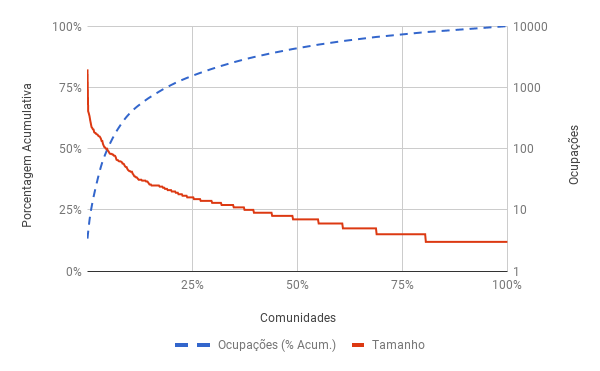
\includegraphics[width=0.9\linewidth]{pareto-comunidades.png}
    \caption{Gráfico de Pareto com a distribuição de tamanho das ilhas ocupacionais. As comunidades estão ordenadas pelo número de ocupações que contêm, ilhas maiores estão à esquerda e menores à direita. O eixo direito, em escala logarítmica, está associado à linha cheia e representa o número de ocupações da ilha. O eixo esquerdo está associado à linha tracejada e representa o total de ocupações e qual a contribuição acumulativa das ilhas à esquerda do ponto para ela.}
    \label{fig:pareto-comunidades}
\end{figure}

%% A QUE RESOLUÇÃO VOCÊ SE REFERE NO PARÁGRAFO ACIMA?
% Ronie (retirei o parágrafo): Limite de Resolução é uma limitação dos algoritmos de detecção de comunidade. Dependendo do algoritmo, ele não é capaz de separar algumas comunidades simplesmente por causa do tamanho da rede ou do número de conexões. Como a maior parte desses algoritmos parte de uma função de otimização global, isso significa que o número relativo de links decide se é melhor uma comunidade estar separada ou junta. Com muito poucas conexões, a função sempre decide por juntar com uma comunidade maior. Na prática, se eu diminuir o tamanho da rede em partes que não interessam, uma comunidade pode 'surgir', apenas pelo todo ter menos conexões. É um problema bem chatinho e algoritmos diferentes podem ter limites de resolução causados por coisas diferentes. No caso do Infomap, o limite tem a ver com o fluxo inter-comunidades (não lembro os detalhes agora, mas o trabalho do Kuwamoto explica isso).

As comunidades, em sua maioria, possuem uma topologia em que predomina a forma de estrela ou estrelas com múltiplos centros. Isso significa poucos \textit{hubs} conectando quase todos os outros nós. Esse formato é caracterizado por uma assortatividade negativa, ou seja, nós de alto grau conectados a nós de baixo grau~\cite{Barabasi2016-rn}.

A assortatividade das 162 ilhas com ao menos três ocupações é exibida na Figura~\ref{fig:assortatividade}. Quase todas elas possuem assortatividade negativa, embora essa característica seja suavizada em ilhas ocupacionais maiores.

A assortatividade negativa confirma a existência de polos ocupacionais para grande parte das ilhas. Na Figura~\ref{fig:ex-ilhas-ocupacionais} são apresentados três exemplos emblemáticos sobre a assortatividade e o efeito esperados dos polos.

\begin{figure}[htb]
    \centering
    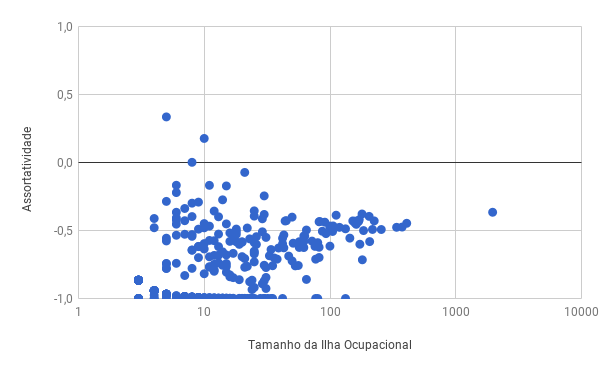
\includegraphics[width=0.9\linewidth]{assortatividade.png}
    \caption{Assortatividade pelo número de ocupações na ilha com o eixo $x$ em escala logarítmica.}
    \label{fig:assortatividade}
\end{figure}

%% PRECISAMOS MOSTRAR E DISCUTIR ALGUNS EXEMPLOS DE COMUNIDADES AQUI. VAMOS DEBATER SEUS COMENTÁRIOS ABAIXO E DEFINIR ALGUNS CAMINHOS PARA FECHARMOS O TRABALHO
% Ronie: Acredito que resolvemos isso na vez que conversamos no LCoN, certo? Incorporei o que entendi da conversa nessa versão :)

A ilha que se inicia com \enquote{Aluno de Iniciação Científica} é exibida na Figura~\ref{fig:ex-sobreposicao-ciencia}. A topologia estrelada é claramente observável, irradiando-se a partir do \textit{polo ocupacional}. O fluxo predominante parte de \textit{Aluno de Iniciação Científica}, passa por \textit{Aluno de Mestrado} e termina em \textit{Aluno de Doutorado} sem que haja fluxo na direção contrária, reforçando o conhecimento tácito sobre a área.

O polo ocupacional é claramente \textit{Aluno de Iniciação Científica}. O reforço dessa ocupação deve distribuir o fluxo de pessoas para as outras ocupações, em especial o fluxo mais forte \textit{Aluno de Mestrado} $\rightarrow$ \textit{Aluno de Doutorado}. Por outro lado, seu enfraquecimento tende a minar o fluxo de pessoa para outras ocupações, provocando o enfraquecimento da ilha como um todo.

Essa análise pontual dá dimensão à contribuição desse trabalho. Nesse caso, identificada a ilha, o polo e o fluxo predominante,  ações para reforçar uma ocupação, como \textit{Aluno de Doutorado}, por exemplo, passam a ser óbvias. Essa análise superficial sugere que aumentar o número de alunos de iniciação científica, desestimular sua movimentação para outras ocupações ou incentivar o fluxo para o mestrado provocaria o efeito desejado. A proporção de pessoas em cada fluxo fornece um \enquote{funil} para se estimar quantas pessoas seriam necessárias em cada ocupação para atingir um certo resultado.

As proporções entre as ocupações, por exemplo, entre \textit{Aluno de Iniciação Científica}, \textit{Aluno de Mestrado} e \textit{Aluno de Doutorado} também podem servir como comparativo entre uma instituição de ensino e o \enquote{mercado}.

A ilha ocupacional relacionada à \textit{Tecnologia da Informação}, exibida na Figura~\ref{fig:ex-sobreposicao-ti}, possui uma topologia de estrela com três polos claros: \textit{Gerente de Projetos}, \textit{Analista de Sistemas} e \textit{Analista de Suporte}. Cada um deles funciona como centro de seu próprio conjunto de ocupações, mas com grande movimentação de profissionais entre si.

A remoção de um desses polos desconectaria a parte das ocupações em que esse polos são a única conexão com a ilha ocupacional, mas não seria suficiente para esfacelá-la como no caso anterior. A conexão de maior fluxo nessa ilha está entre \textit{Analista de Suporte} $\rightarrow$ \textit{Analista de Sistemas}. Chama a atenção não haver um fluxo direto significativo entre \textit{Analista de Suporte} e \textit{Gerente de Projetos}, indicando que \textit{Analista de Sistemas} pode funcionar como uma \textit{ponte} entre essas ocupações.

%% EXISTE UM DESEQUILÍBRIO NA PROFUNDIDADE DA EXPLICAÇÃO DO CASO 1 PARA ESTE CASO 2 E O PRÓXIMO, FAVOR BALANCEAR.
% Ronie: Feito, mas não consegui aprofundar mais.

No último exemplo da Figura~\ref{fig:ex-sobreposicao-vendas}, exibindo a ilha relacionada a \textit{Comercial e Vendas}, os polos não são tão claros. \textit{Gerente Comercial} e \textit{Consultor de Vendas} se destacam, mas quatro outros nós possuem grande fluxo e alta conectividade. A remoção de um desses nós não afetaria a rede da mesma forma que nos exemplos anteriores. Nota-se também que há um forte fluxo entre todos os nós de maior fluxo, diferentemente do exemplo da ilha de \textit{Tecnologia da Informação}, em que dois dos polos possuem conexão tão tênue que não figura entre as conexões de maior fluxo da rede.

A topologia é mais similar a de \textit{centro e raios}, em que as ocupações mais periféricas se conectam entre si, mas ainda assim possuem um grau elevado de conexões.

\begin{figure}[ht]
    \centering
    \subfloat[][Iniciação Científica] {
        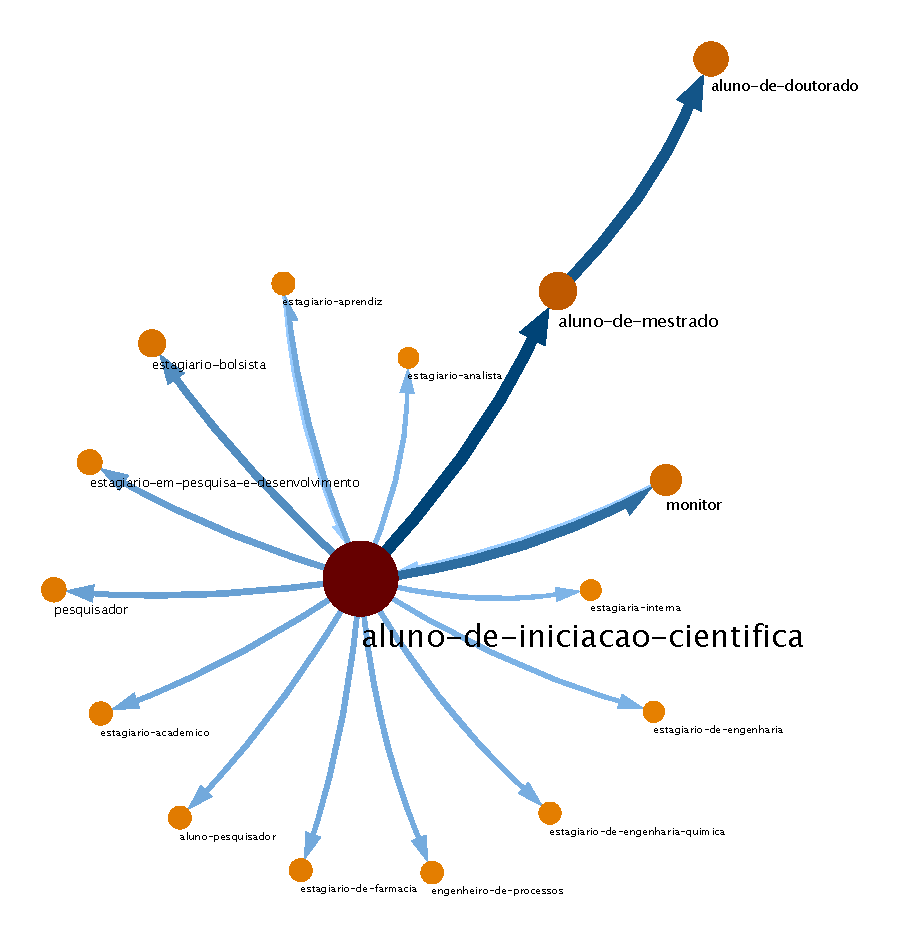
\includegraphics[width=0.5\linewidth]{ex-sobreposicao-aluno-iniciacao.pdf}
        \label{fig:ex-sobreposicao-ciencia}
    }
    \subfloat[][Tecnologia da Informação] {
        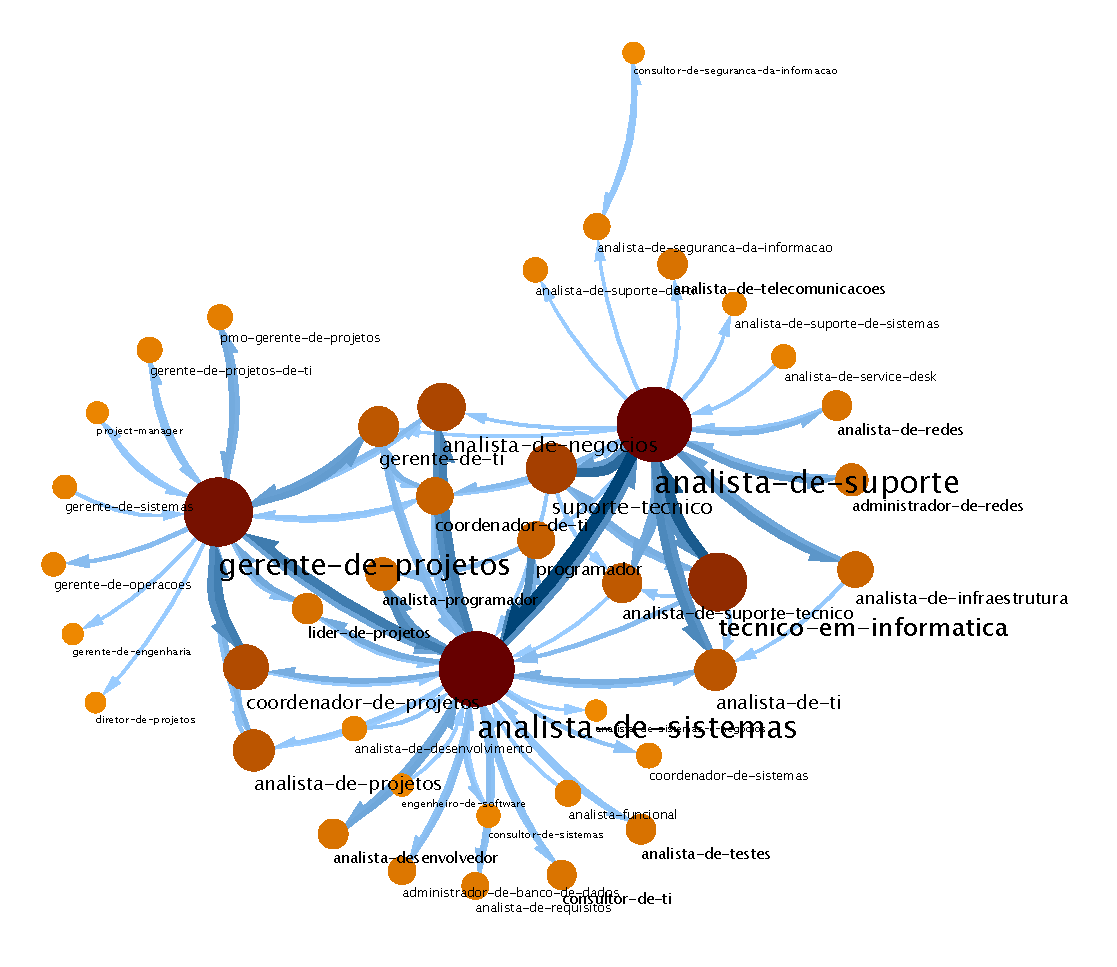
\includegraphics[width=0.5\linewidth]{ex-sobreposicao-analista-de-sistemas.pdf}
        \label{fig:ex-sobreposicao-ti}
    }
    \\    
    \subfloat[][Comercial e Vendas] {
        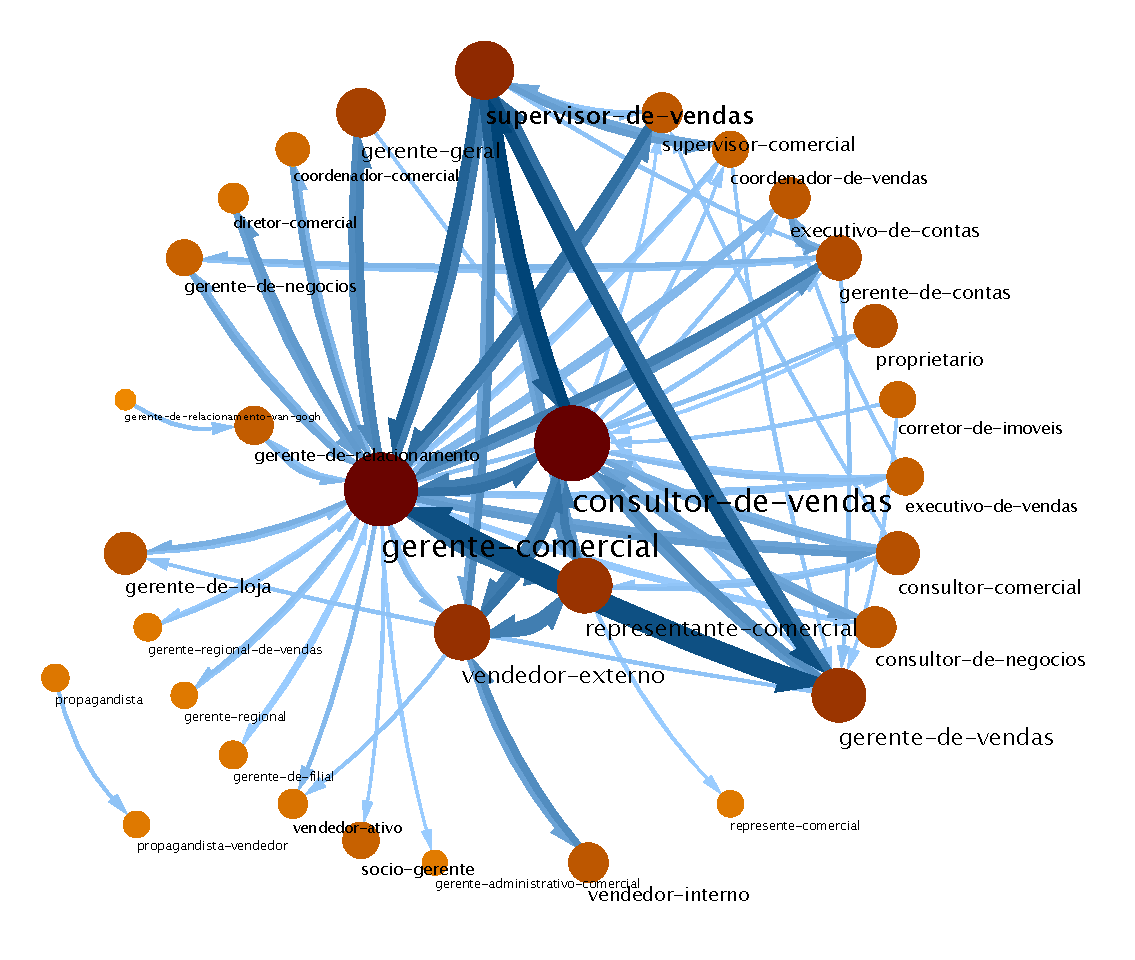
\includegraphics[width=0.5\linewidth]{ex-sobreposicao-consultor-de-vendas.pdf}
        \label{fig:ex-sobreposicao-vendas}
    }
    \caption{Três exemplos de ilhas ocupacionais. O tamanho e a cor do nó estão relacionados ao fluxo de profissionais que passa por ele, quanto maior e mais escuro o nó, maior o fluxo. Da mesma forma, a espessura e a cor das conexões está relacionada ao fluxo de profissionais entre uma ocupação e outra. O polos ocupacionais são identificados pelo volume de pessoas transitando por eles e pela sua alta conectividade (visualmente os nós maiores e mais centrais). Para facilitar a visualização, nas Figuras~\ref{fig:ex-sobreposicao-ti} e~\ref{fig:ex-sobreposicao-vendas}, apenas as conexões e nós de maior fluxo são apresentados. A Figura~\ref{fig:ex-sobreposicao-ciencia}, no entanto, mostra a ilha completa.}
    \label{fig:ex-ilhas-ocupacionais}
\end{figure}

%===================================
\section{Conclusões e Perspectivas Futuras}
%===================================

Esse trabalho reúne os conceitos fronteiras de carreira de \citeonline{Gunz2007-hr}, os trabalhos de Ciência de Redes sobre detecção de comunidades por fluxo baseados em \cite{Rosvall2009-sd} e os dados de um dos maiores sites brasileiros de carreira~\cite{VAGAS_Tecnologia2014-yv} para contribuir na compreensão da movimentação profissional.

A rede profissional possui \textit{hubs}, o que fornece indícios de que carreiras menos regulares são comuns, como advogam as Carreiras sem Fronteiras e Carreiras Proteanas, ao mesmo tempo que sugerem que eles possuem limitações.

O algoritmo Infomap foi aplicado para identificar as fronteiras de carreiras, gerando \textit{ilhas ocupacionais}, que são conjuntos de ocupações em que a movimentação interna é significativamente mais frequente do que movimentações para outras \textit{ilhas}. O termo foi introduzido para facilitar a discussão e como uma analogia ao conceito sugerido por~\cite{Abbott1995-ft} em que a fronteira define o grupo, ao invés do grupo definir a fronteira.

A análise da assortatividade das ilhas mostrou que sua topologia tende ao formato estrelado ou de eixo e raios, o que motivou a introdução do termo \textit{polos ocupacionais} para identificar ocupações que dão coesão à ilha. Alguns exemplos emblemáticos dão dimensão aos dois conceitos introduzidos nesse trabalho.

Conclui-se na expectativa que esse trabalho contribua para na compreensão das transições profissionais, no entanto, é preciso reconhecer as limitações dessa proposta e as questões que permanecem abertas.

%% OPS, SIM, É VERDADE, MAS NÃO PODEMOS USAR ESSA REDAÇÃO EM UM ARTIGO CIENTÍFICO. PODEMOS DIZER, POR EXEMPLO, "ESSE TRABALHO TRAZ UMA IMPORTANTE CONTRIBUIÇÃO PARA O ENTENDIMENTO DAS MOVIMENTAÇÕES DE CARREIRA USANDO UMA BASE DE DADOS REAL E CONCEITOS DE CIÊNCIA DE REDES, E ABRE DIVERSAS PERSPECTIVAS RELEVANTES DE PESQUISA..."
% Ronie: Feito

%% NORMALMENTE AS CONCLUSÕES INICIAM FAZENDO UMA BREVE REVISÃO DE TUDO QUE FOI APRESENTADO, PARTINDO DAS HIPÓTESES DE PESQUISA, ATÉ AS CONCLUSÕES OBTIDAS. A PARTIR DISSO QUE INSERIMOS AS PERSPECTIVAS FUTURAS.
% Ronie: Feito

Os aspectos sociais e psicológicos das fronteiras de carreira não foram abordados e são eles quem podem responder a perguntas como \enquote{por que as fronteiras estão onde estão?} e \enquote{por que as ilhas possuem essa topologia?}. Espera-se que o conteúdo apresentado contribua de maneira quantitativa em discussões sociais e psicológicas sobre movimentação profissional.

Outros trabalhos podem aprofundar a questão da dinâmica da rede, focando em modelos que possam predizer os efeitos esperados quando uma ocupação ganha ou perde atratividade, ou quando um fluxo é incentivado ou estrangulado. Esse trabalho ensaia um começo tímido nessa direção ao propor o conceito de polos ocupacionais e identificar sua importância nas ilhas de ocupações.

Outra linha de pesquisa atrativa está em comparar o MCar com redes aleatórias geradas a partir de características similares à da rede real, procurando identificar quais delas resultam em observações comparáveis. Essas características indicam possíveis explicações para os comportamentos encontrados a partir de uma abordagem puramente estatística~\cite{Barabasi2016-rn}.

O MCar é uma fonte considerável de informação sobre o mercado de trabalho brasileiro. Outras pesquisas sobre profissões e carreira, em especial utilizando técnicas de Ciência de Redes, como \textit{motifs}, podem contribuir para uma melhor compreensão da movimentação profissional.

\newpage

\bibliography{main}
\end{document}
